\documentclass[11pt,letterpaper]{article}
\usepackage[lmargin=1in,rmargin=1in,tmargin=1in,bmargin=1in]{geometry}
\usepackage{../style/homework}
\usepackage{../style/commands}
\setbool{quotetype}{false} % True: Side; False: Under
\setbool{hideans}{false} % Student: True; Instructor: False

% -------------------
% Content
% -------------------
\begin{document}

\homework{21: Due 12/15}{All paths are not equal; if they were, they wouldn't be paths but rather the points at each end.}{H.E. Huntley}

% Problem 1
\problem{10} Does the graph $G$ below have an Euler circuit or Euler trail? If it has an Euler circuit or Euler trail, find it. If it does not have an Euler circuit or Euler trail, explain why not. 
	\[
	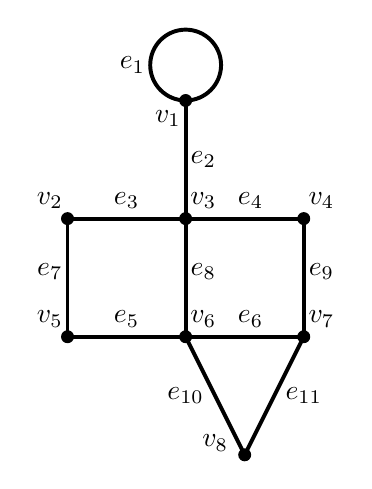
\begin{tikzpicture}[scale=1.5]
	\draw[line width=0.05cm] (0,2.3) circle (0.3);
	\draw[line width=0.05cm] (0,2) to (0,1);
	\draw[line width=0.05cm] (-1,1) to (1,1);
	\draw[line width=0.05cm] (-1,0) to (1,0);
	\draw[line width=0.05cm] (-1,1) to (-1,0);
	\draw[line width=0.05cm] (1,1) to (1,0);
	\draw[line width=0.05cm] (0,1) to (0,0);
	\draw[line width=0.05cm] (0,0) to (0.5,-1);
	\draw[line width=0.05cm] (1,0) to (0.5,-1);
	
	\draw[fill= black] (0,2) circle (0.05);
	\draw[fill= black] (-1,1) circle (0.05);
	\draw[fill= black] (0,1) circle (0.05);
	\draw[fill= black] (1,1) circle (0.05);
	\draw[fill= black] (-1,0) circle (0.05);
	\draw[fill= black] (0,0) circle (0.05);
	\draw[fill= black] (1,0) circle (0.05);
	\draw[fill= black] (0.5,-1) circle (0.05);
	
	\node at (-0.15,1.85) {$v_1$};
	\node at (-1.15,1.15) {$v_2$};
	\node at (0.15,1.15) {$v_3$};
	\node at (1.15,1.15) {$v_4$};
	\node at (-1.15,0.15) {$v_5$};
	\node at (0.15,0.15) {$v_6$};
	\node at (1.15,0.15) {$v_7$};
	\node at (0.25,-0.90) {$v_8$};

	\node at (-0.45,2.3) {$e_1$};
	\node at (0.15,1.5) {$e_2$};
	\node at (-0.5, 1.15) {$e_3$};
	\node at (0.55,1.15) {$e_4$};
	\node at (-0.5,0.15) {$e_5$};
	\node at (0.55,0.15) {$e_6$};
	\node at (-1.15,0.55) {$e_7$};
	\node at (0.15,0.55) {$e_8$};
	\node at (1.15,0.55) {$e_9$};
	\node at (0,-0.5) {$e_{10}$};
	\node at (1,-0.5) {$e_{11}$};
	\end{tikzpicture}
	\] \pspace

\sol An undirected graph $G$ has an Euler circuit if and only if $G$ is connected and every vertex has positive even degree. The graph $G$ is connected because given any two vertices there is a walk between them. However, the vertex $v_7$ has odd degree---we have $\deg v_7= 3$. Therefore, $G$ does not have an Euler circuit. \pspace

An undirected graph $G$ has an Euler trail if and only if $G$ is connected and it has exactly two vertices of odd degree. The graph $G$ is connected because given any two vertices there is a walk between them. Observe that $\deg v_1= 3$ (the loop contributes 2 to the degree) and $\deg v_7= 3$. All other vertices of $G$ have even degree. Therefore, $G$ has an Euler trail. For instance, the following is an Euler trail:
	\[
	v_7 \, e_{11} \, v_8 \, e_{10} \, v_6 \, e_6 \, v_7 \, e_9 \, v_4 \, e_4 \, v_3 \, e_3 \, v_2 \, e_7 \, v_5 \, e_5 \, v_6 \, e_8 \, v_3 \, e_2 \, v_1 \, e_1
	\]



\newpage



% Problem 2
\problem{10} Let $G$ be the graph given below.
	\[
	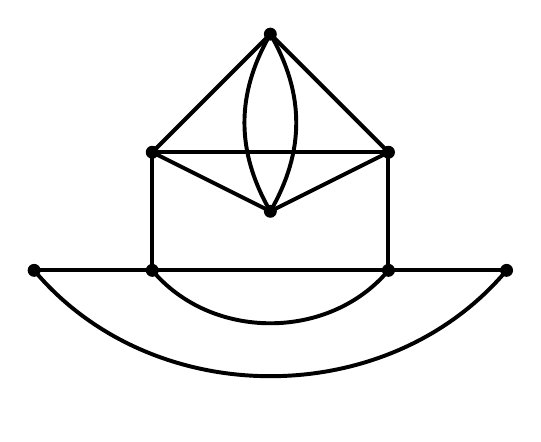
\begin{tikzpicture}[scale=1.5]
	\draw[line width=0.05cm] (-2,0) to (2,0);
	\draw[line width=0.05cm] (-1,0) to (-1,1);
	\draw[line width=0.05cm] (1,0) to (1,1);
	\draw[line width=0.05cm] (-1,1) to (1,1);
	\draw[line width=0.05cm] (-1,1) to (0,2);
	\draw[line width=0.05cm] (1,1) to (0,2);
	\draw[line width=0.05cm] (-1,1) to (0,0.5);
	\draw[line width=0.05cm] (1,1) to (0,0.5);
	\draw[line width=0.05cm, bend right=50] (-1,0) to (1,0);
	\draw[line width=0.05cm, bend right=50] (-2,0) to (2,0);
	\draw[line width=0.05cm, bend right= 30] (0,2) to (0,0.5);
	\draw[line width=0.05cm, bend left= 30] (0,2) to (0,0.5);
	
	\draw[fill= black] (0,2) circle (0.05);
	\draw[fill= black] (-1,1) circle (0.05);
	\draw[fill= black] (1,1) circle (0.05);
	\draw[fill= black] (0,0.5) circle (0.05);
	\draw[fill= black] (-2,0) circle (0.05);
	\draw[fill= black] (-1,0) circle (0.05);
	\draw[fill= black] (1,0) circle (0.05);
	\draw[fill= black] (2,0) circle (0.05);
	\end{tikzpicture}
	\]
\begin{enumerate}[(a)]
\item Does $G$ have an Euler trail? If it does, find it. If it does not, explain why. 
\item Does $G$ have a Hamiltonian circuit? If it does, find it. If it does not, explain why. 
\end{enumerate} \pspace

\sol 
\begin{enumerate}[(a)]
\item A graph $G$ has an Euler trail if and only if it is connected and every vertex has positive even degree. The graph $G$ is connected because every pair of vertices has a walk from one to the other. Furthermore, every vertex of $G$ has degree 4 except the `leftmost' and `rightmost' vertices which have degree 2. Therefore, $G$ does not have an Euler trail. \pspace

\item A Hamiltonian circuit is a walk which visits every vertex precisely once and starts/ends at the same vertex. The graph $G$ has a Hamiltonian circuit. For instance, there is a Hamiltonian circuit highlighted in red in the graph below:
	\[
	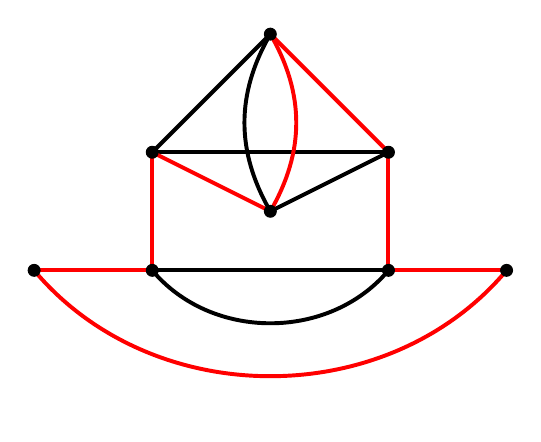
\begin{tikzpicture}[scale=1.5]
	\draw[line width=0.05cm,red] (-2,0) -- (-1,0);
	\draw[line width=0.05cm] (-1,0) -- (1,0);
	\draw[line width=0.05cm,red] (1,0) -- (2,0);
	\draw[line width=0.05cm,red] (-1,0) to (-1,1);
	\draw[line width=0.05cm,red] (1,0) to (1,1);
	\draw[line width=0.05cm] (-1,1) to (1,1);
	\draw[line width=0.05cm] (-1,1) to (0,2);
	\draw[line width=0.05cm,red] (1,1) to (0,2);
	\draw[line width=0.05cm,red] (-1,1) to (0,0.5);
	\draw[line width=0.05cm] (1,1) to (0,0.5);
	\draw[line width=0.05cm, bend right=50] (-1,0) to (1,0);
	\draw[line width=0.05cm, bend right=50,red] (-2,0) to (2,0);
	\draw[line width=0.05cm, bend right= 30] (0,2) to (0,0.5);
	\draw[line width=0.05cm, bend left= 30,red] (0,2) to (0,0.5);
	
	\draw[fill= black] (0,2) circle (0.05);
	\draw[fill= black] (-1,1) circle (0.05);
	\draw[fill= black] (1,1) circle (0.05);
	\draw[fill= black] (0,0.5) circle (0.05);
	\draw[fill= black] (-2,0) circle (0.05);
	\draw[fill= black] (-1,0) circle (0.05);
	\draw[fill= black] (1,0) circle (0.05);
	\draw[fill= black] (2,0) circle (0.05);
	\end{tikzpicture}
	\]
\end{enumerate}





\newpage



% Problem 3
\problem{10} Suppose $G$ is the graph given below on the left and that $H$ is a directed graph with adjacency matrix $A$. Showing all your work and fully justifying your responses, answer the questions below. \par
	\begin{minipage}[c]{0.49\textwidth}
	\[
	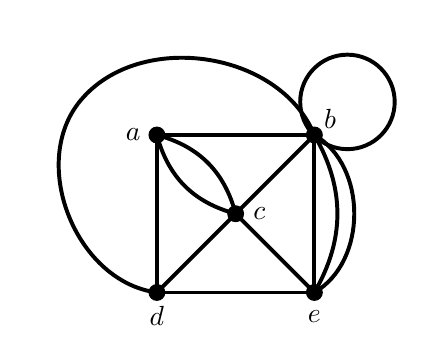
\begin{tikzpicture}[scale=2]
	\draw[line width=0.05cm] (0,0) to (1,0);
	\draw[line width=0.05cm] (0,0) to (0,1);
	\draw[line width=0.05cm] (0,1) to (1,1);
	\draw[line width=0.05cm] (1,0) to (1,1);
	\draw[line width=0.05cm] (0,0) to (1,1);
	\draw[line width=0.05cm] (0.5,0.5) to (1,0);
	\draw[line width=0.05cm, bend right= 30] (0,1) to (0.5,0.5);
	\draw[line width=0.05cm, bend left= 30] (0,1) to (0.5,0.5);
	\draw[line width=0.05cm, bend right= 30] (1,0) to (1,1);
	\draw[line width=0.05cm, bend right= 60] (1,0) to (1,1);
	\draw[line width=0.05cm, bend left= 60] (0,0) to (-0.5,1.2);
	\draw[line width=0.05cm, bend right= 60] (1,1) to (-0.5,1.2);
	\draw[line width=0.05cm] (1.21,1.21) circle (0.3);
	
	\draw[fill= black] (0,0) circle (0.05);
	\draw[fill= black] (1,0) circle (0.05);
	\draw[fill= black] (1,1) circle (0.05);
	\draw[fill= black] (0,1) circle (0.05);
	\draw[fill= black] (0.5,0.5) circle (0.05);
	
	\node at (-0.15,1) {$a$};
	\node at (1.10,1.10) {$b$};
	\node at (0.65,0.50) {$c$};
	\node at (0,-0.15) {$d$};
	\node at (1,-0.15) {$e$};
	\end{tikzpicture}
	\]
	\end{minipage}%
	\begin{minipage}[c]{0.49\textwidth}
	\[
	A^8= 
	\begin{pmatrix}
	408 628 & 1456983 & 1201872 & 1045608 \\
	217055 & 774044 & 638429 & 555540 \\
	442957 & 1577690 & 1299626 & 1131303 \\
	280444 & 1001303 & 825067 & 716683
	\end{pmatrix}
	\]
	\end{minipage}

\begin{enumerate}[(a)]
\item How many walks are there of length 1 from $b$ to $e$? What about from $d$ to $b$?
\item How many walks are there of length 2 from $c$ to itself? What about from $e$ to $a$?
\item How many walks are there of length 4 from $a$ to $c$? What about from $b$ to itself?
\item How many connected components does $G$ have?
\item How many walks are there of length 8 from $v_1$ to $v_3$ in $H$? What about $v_4$ to $v_2$?
\end{enumerate} \pspace

\sol 
\begin{enumerate}[(a)]
\item The number of walks of length $k$ in a graph $G$ from $v_i$ to $v_j$ is the entry $a_{ij}$ in $A^k$, where $A$ is the adjacency matrix of $G$. The adjacency matrix of $G$ is\dots
	\[
	A= 
	\begin{pmatrix}
	0 & 1 & 2 & 1 & 0 \\
	1 & 1 & 1 & 1 & 3 \\
	2 & 1 & 0 & 1 & 1 \\
	1 & 1 & 1 & 0 & 1 \\
	0 & 3 & 1 & 1 & 0 
	\end{pmatrix}
	\]
The number of walks of length 1 from $b$ to $e$ is $a_{2,5}= 3$. The number of walks of length 1 from $d$ to $b$ is $a_{4,2}= 1$. \pspace

\item The number of walks of length 2 from $v_i$ to $v_j$ is the entry $a_{ij}$ in $A^2$. We have\dots
	\[
	A^2= 
	\begin{pmatrix}
	0 & 1 & 2 & 1 & 0 \\
	1 & 1 & 1 & 1 & 3 \\
	2 & 1 & 0 & 1 & 1 \\
	1 & 1 & 1 & 0 & 1 \\
	0 & 3 & 1 & 1 & 0 
	\end{pmatrix}
	\begin{pmatrix}
	0 & 1 & 2 & 1 & 0 \\
	1 & 1 & 1 & 1 & 3 \\
	2 & 1 & 0 & 1 & 1 \\
	1 & 1 & 1 & 0 & 1 \\
	0 & 3 & 1 & 1 & 0 
	\end{pmatrix}= 
	\begin{pmatrix}
	6 & 4 & 2 & 3 & 6 \\
	4 & 13 & 7 & 6 & 5 \\
	2 & 7 & 7 & 4 & 4 \\
	3 & 6 & 4 & 4 & 4 \\
	6 & 5 & 4 & 4 & 11
	\end{pmatrix}
	\]
But then the number of walks of length 2 from $c$ to $c$ is $a_{3,3}= 7$. The number of walks of length 2 from $e$ to $a$ is $a_{5,1}= 6$. 

\item The number of walks of length 4 from $v_i$ to $v_j$ is the entry $a_{ij}$ in $A^4= (A^2)^2$. We have\dots
	\[
	A^4= (A^2)^2= 
	\begin{pmatrix}
	6 & 4 & 2 & 3 & 6 \\
	4 & 13 & 7 & 6 & 5 \\
	2 & 7 & 7 & 4 & 4 \\
	3 & 6 & 4 & 4 & 4 \\
	6 & 5 & 4 & 4 & 11
	\end{pmatrix}
	\begin{pmatrix}
	6 & 4 & 2 & 3 & 6 \\
	4 & 13 & 7 & 6 & 5 \\
	2 & 7 & 7 & 4 & 4 \\
	3 & 6 & 4 & 4 & 4 \\
	6 & 5 & 4 & 4 & 11
	\end{pmatrix}=
	\begin{pmatrix}
	101 & 138 & 90 & 86 & 142 \\
	138 & 295 & 192 & 162 & 196 \\
	90 & 192 & 134 & 108 & 135 \\
	86 & 162 & 108 & 93 & 124 \\
	142 & 196 & 135 & 124 & 214
	\end{pmatrix}
	\]
Therefore, the number of walks of length 4 from $a$ to $c$ is $a_{1,3}= 90$. The number of walks of length 4 from $b$ to itself is $a_{2,2}= 295$. \pspace
 
\item The graph $G$ is connected because every two distinct vertices in $G$ has a walk connecting them. Therefore, $G$ has one connected component. \pspace

\item The number of walks of length 8 from $v_i$ to $v_j$ is the entry $a_{ij}$ in $A^8$, where $A$ is the adjacency matrix of the graph. But then the number of walks of length 8 from $v_1$ to $v_3$ in $H$ is $a_{1,3}= 1201872$. The number of walks of length 8 from $v_4$ to $v_2$ is $a_{4,2}= 1001303$. 
\end{enumerate}



\newpage



% Problem 4
\problem{10} Suppose that $G$ is an undirected graph with adjacency matrix, $A$, given below. 
	\[
	A= 
	\begin{pmatrix}
	0 & 2 & 1 & 0 & 0 & 0 & 0 & 0 \\
	2 & 0 & 1 & 0 & 0 & 0 & 0 & 0 \\
	1 & 1 & 0 & 0 & 0 & 0 & 0 & 0 \\
	0 & 0 & 0 & 0 & 1 & 0 & 0 & 0 \\
	0 & 0 & 0 & 1 & 1 & 2 & 0 & 0 \\
	0 & 0 & 0 & 0 & 2 & 0 & 0 & 0 \\
	0 & 0 & 0 & 0 & 0 & 0 & 0 & 0 \\
	0 & 0 & 0 & 0 & 0 & 0 & 0 & 1
	\end{pmatrix}
	\]
Using only this adjacency matrix, showing all your work, fully justifying your responses, answer the following:
\begin{enumerate}[(a)]
\item Is $G$ a simple graph?
\item Is $G$ a multigraph?
\item How many connected components does $G$ have?
\item Find the degrees of vertices $v_1$, $v_8$, and $v_5$.
\item What is the degree of $G$?
\end{enumerate} \pspace

\sol 
\begin{enumerate}[(a)]
\item A graph $G$ is simple if and only if it does not have loops or multiple edges. A loop is an edge from a vertex to itself. But this occurs if and only if $A_{i,i} > 0$. Because $A_{5,5} > 0$, there is a loop at $v_5$. Therefore, $G$ is not simple. A graph has multiple edges if and only if there exist two distinct vertices with more than one edge between them. But this occurs if and only if $A_{i,j} > 1$ for some $i, j$. Because $A_{1,2}= 2 > 1$, there are two edges from $v_1$ to $v_2$. But then $G$ is not simple. \pspace

\item A graph $G$ is a multigraph if and only if there exist two distinct vertices with more than one edge between them. But this occurs if and only if $A_{i,j} > 1$ for some $i, j$. Because $A_{1,2}= 2 > 1$, there are two edges from $v_1$ to $v_2$. But then $G$ is a multigraph. \pspace

\item The number of connected components is the number of blocks in its adjacency matrix. Observe that we can block $A$ as follows:
	\[
	A= 
	\begin{pmatrix}[ccc|ccc|c|c]
	0 & 2 & 1 & 0 & 0 & 0 & 0 & 0 \\
	2 & 0 & 1 & 0 & 0 & 0 & 0 & 0 \\
	1 & 1 & 0 & 0 & 0 & 0 & 0 & 0 \\ \hline
	0 & 0 & 0 & 0 & 1 & 0 & 0 & 0 \\
	0 & 0 & 0 & 1 & 1 & 2 & 0 & 0 \\
	0 & 0 & 0 & 0 & 2 & 0 & 0 & 0 \\ \hline
	0 & 0 & 0 & 0 & 0 & 0 & 0 & 0 \\ \hline
	0 & 0 & 0 & 0 & 0 & 0 & 0 & 1
	\end{pmatrix}
	\]
Therefore, there are 4 connected components. \pspace

\item The degree of a vertex from its adjacency matrix can be found by summing the entries in its row---being sure to count loops, i.e. entries along the diagonal, twice. But then we have $\deg v_1= 2 + 1= 3$, $\deg v_8= 2 \cdot 1= 2$, and $\deg v_5= 1 + 2 \cdot 1 + 2= 5$. \pspace

\item The degree of $G$ is the sum of the degrees of its vertices. Using the procedure outlined in (d), we have\dots
	\[
	\deg G= \sum_{v_i} \deg v_i= 3 + 3 + 2 + 1 + 5 + 2 + 0 + 2= 18
	\]
Alternatively, because $G$ is undirected, we can use the Handshake Theorem. The degree of $G$ is twice the number of edges. The number of edges is the sum of all the entries on or above the diagonal. But then we have $\deg G= 2 |E(G)|= 2 (1 + 1 + 2 + 1 + 1 + 2 + 1)= 2 \cdot 9= 18$. 
\end{enumerate}















\end{document}